\documentclass[12pt]{report}
\usepackage{./sty/dissert}% style
\usepackage{comment}
\usepackage{hyperref}
\usepackage[acronym]{glossaries}
\usepackage{titlesec}
\usepackage{xcolor}
\usepackage{graphicx}
\usepackage{fancyhdr}
\usepackage{lastpage}
\usepackage{listings}
\usepackage{lmodern}
\usepackage[portuguese]{babel}

\lstdefinestyle{codigo}{
    basicstyle=\ttfamily\scriptsize,      
    columns=fullflexible,                 
    keepspaces=true,                      
    keywordstyle=\color{blue!70!black}\bfseries,
    commentstyle=\color{green!45!black}\itshape,
    stringstyle=\color{red!65!black},
    numbers=left, numberstyle=\tiny\color{gray}, numbersep=4pt,                        
    frame=single,
    framesep=2pt,                         
    aboveskip=4pt, belowskip=2pt,         
    xleftmargin=2pt, xrightmargin=2pt,    
    rulecolor=\color{gray!40},
    backgroundcolor=\color{gray!6},
    breaklines=true,
    showstringspaces=false,
    tabsize=2,                            
    captionpos=b,
    literate={á}{{\'a}}1 {é}{{\'e}}1 {í}{{\'i}}1 {ó}{{\'o}}1 {ú}{{\'u}}1
             {ã}{{\~a}}1 {õ}{{\~o}}1 {ç}{{\c{c}}}1 {â}{{\^a}}1 {ê}{{\^e}}1
}
\lstset{style=codigo}
\captionsetup[lstlisting]{skip=2pt}

% Portuguese names
\renewcommand{\lstlistingname}{Código}
\renewcommand{\lstlistlistingname}{Lista de Códigos}
\hypersetup{
    colorlinks,
    linkcolor={black!50!black},
    citecolor={black!50!black},
    urlcolor={black!80!black}
}
\titleformat{\chapter}{\LARGE}{\thechapter.}{20pt}{\LARGE\textbf}
\titlespacing*{\chapter}{0pt}{0pt}{20pt}
\renewcommand{\figurename}{Figura}
\titleformat*{\section}{\large\bfseries}
%
\makeglossaries%
 % ------------------- Document -----------------------------------------------------
\begin{document}
%\onehalfspacing
\pagenumbering{roman}
\newcommand\tab[1][1cm]{\hspace*{#1}}
%
\setlength{\headheight}{28pt}   
\pagestyle{fancy}
\fancyhf{}                   

% ---- Header ----
\fancyhead[L]{
\includegraphics[height=0.8cm]{img/logo.png}}
\fancyhead[C]{Observadores Hands-On}
\fancyhead[R]{\leftmark}        

% ---- Footer (rodapé) ----
\fancyfoot[L]{Nuno Costa PG63901}
\fancyfoot[C]{Página \thepage\ de \pageref{LastPage}}
\fancyfoot[R]{Fábio Alves PG63877}

% ---- Lines ----
\renewcommand{\headrulewidth}{0.4pt}   
\renewcommand{\footrulewidth}{0.4pt}  
% --------------TRABALHO------------------
\pagenumbering{arabic}

% Ex 1 %%%%%%%%%%%%%%%%%%%%%%%%%%%%
\noindent \textbf{1)}

\textbf{1.1)} Medindo só a posição não nos impede de estimar a velocidade pois as medições são dadas ao longo do tempo, logo é possível obter a sua variação, ou  seja a velocidade, pois $\dot{p}=v$.

\textbf{1.2)} 
\noindent
\begin{minipage}[t]{0.40\textwidth}
Para verificar a observabilidade calcula-se a matriz
$\mathcal{O}$ com \lstinline{obsv()} e compara-se a sua
característica com a ordem do sistema $n$. Como
$\mathrm{rank}(\mathcal{O}) = 2 = n$, o sistema é
observável.
\begin{lstlisting}[language=Matlab, caption={Resultado}, label={lst:obs_result}, numbers=none]
O =
     1     0
     0     1
r =
     2
O sistema é observável
\end{lstlisting}
\end{minipage}
\hfill
\begin{minipage}[t]{0.45\textwidth}
\begin{lstlisting}[language=Matlab]
O = obsv(A, C)
r = rank(O)
if r == n
    fprintf('O sistema é observável\n')
else
    fprintf('O sistema não é observável\n');
end
\end{lstlisting}
\captionof{lstlisting}{Observabilidade}
\label{lst:obsv}

\end{minipage}

\textbf{1.3)} Com $L=0$ a planta é estável ($\operatorname{eig}(A)=-0.75\pm4.41j$), logo o erro decai sozinho, sendo oscilatório, ao ritmo imposto pela planta.

\begin{figure}[htbp]
    \centering
    \begin{subfigure}[b]{0.48\textwidth}
        \centering
        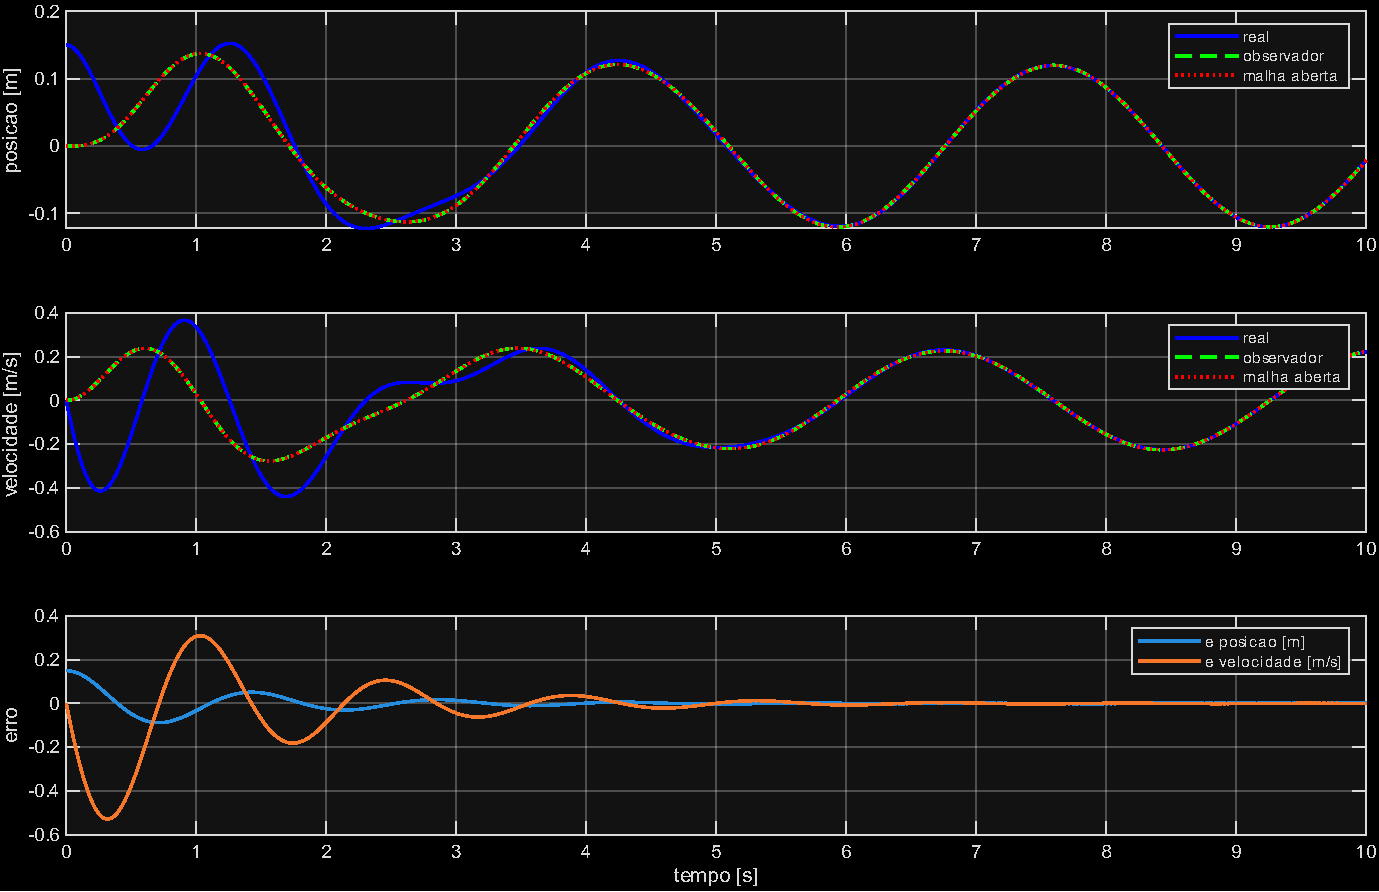
\includegraphics[width=\linewidth]{img/Estados e erro_1.pdf}
        \label{fig:estados1}
    \end{subfigure}
    \hfill
    \begin{subfigure}[b]{0.48\textwidth}
        \centering
        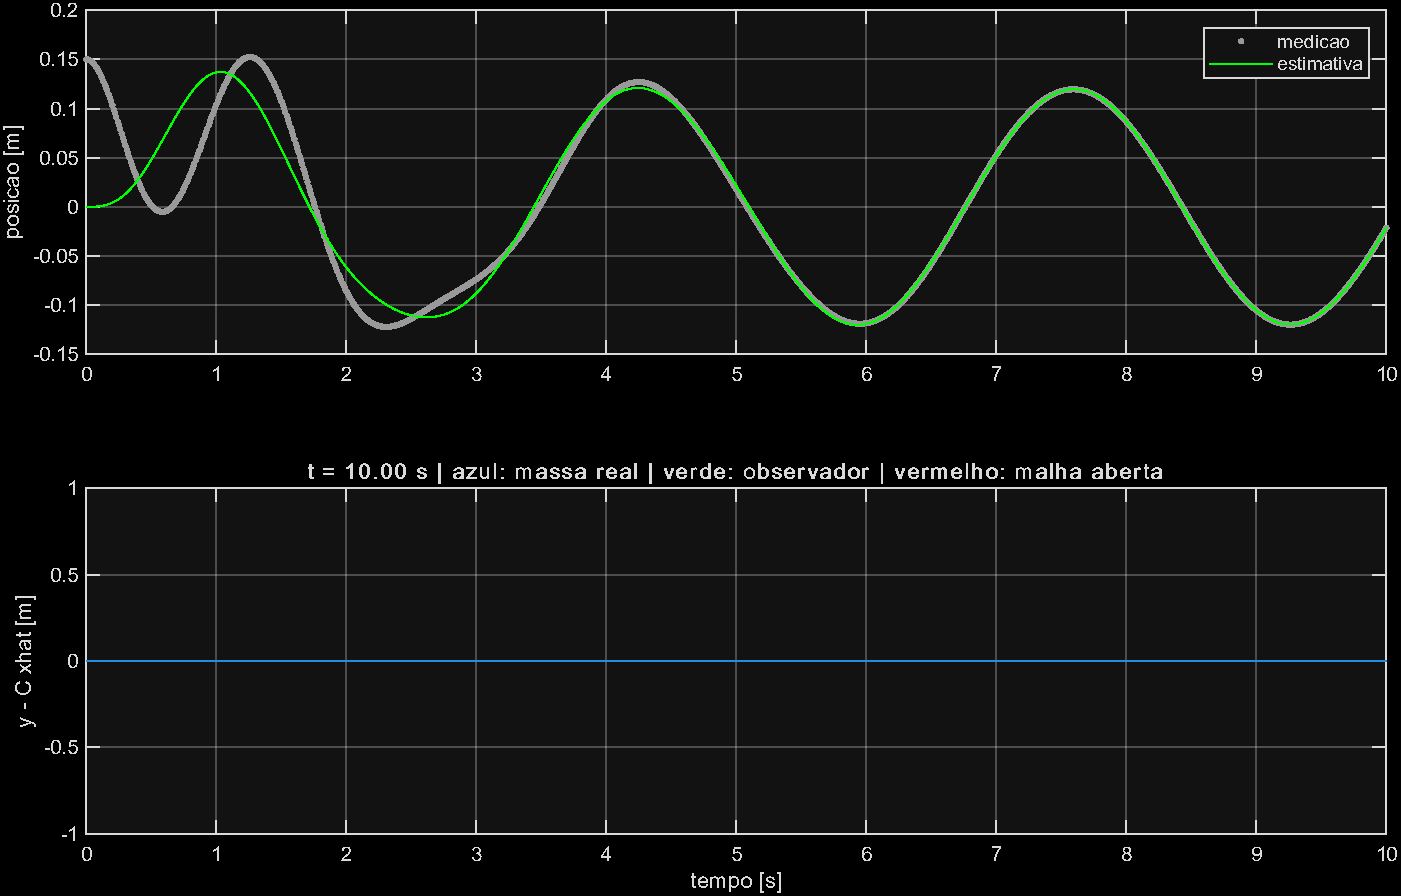
\includegraphics[width=\linewidth]{img/Medicao e inovacao_1.pdf}
        \label{fig:medicao1}
    \end{subfigure}
    \caption{Resultados da simulação com L = 0}
    \label{fig:Simul 1}
\end{figure}

% Ex 2 %%%%%%%%%%%%%%%%%%%%%%%%%%%%
\noindent \textbf{2)}

\textbf{2.1)} Em discreto, a estabilidade é definida pelo módulo dos polos ($|z|<1 =>$ Estável), porém -3 e -4 são polos contínuos, e aplicando a regra: $|-3|>1$ e $|-4|>1$, logo os polos estão fora do círculo unitário, indicando instabilidade.

\textbf{2.2)}
\noindent
\begin{minipage}[t]{0.40\textwidth}
Com os pólos escolhidos, a matriz de ganho do observador é calculada com \lstinline{place()}.
\begin{lstlisting}[language=Matlab, caption={Resultado}, label={lst:obs_result}, numbers=none]
pd =
    0.9704    0.9608
L =
    0.0519
   -0.1663
\end{lstlisting}
\end{minipage}
\hfill
\begin{minipage}[t]{0.45\textwidth}
\begin{lstlisting}[language=Matlab]
pd = exp(cfg.poles*cfg.Ts)
L = place(Ad',Cd',pd)'
\end{lstlisting}
\captionof{lstlisting}{Pólos e ganho do observador}
\label{lst:obsv}

\end{minipage}

\textbf{2.3)}
\begin{minipage}[t]{0.40\textwidth}
$eig$ é igual a $p_d$ (a menos da ordem e de erros numéricos $\approx10^{-10}$, pelo que a comparação se faz com \texttt{sort} e tolerância, não com \texttt{==}).
\begin{lstlisting}[language=Matlab, caption={Resultado}, label={lst:obs_result}, numbers=none]
ei =
    0.9608 
    0.9704
Os pólos coincidem
\end{lstlisting}
\end{minipage}
\hfill
\begin{minipage}[t]{0.45\textwidth}
\begin{lstlisting}[language=Matlab]
ei = eig(Ad-L*Cd)
if abs(sort(ei') - sort(pd)) < 1e-10
    fprintf('Os pólos coincidem\n')
else
    fprintf('Os pólos não coincidem\n')
end
\end{lstlisting}
\captionof{lstlisting}{Comparação de polos}
\label{lst:polos}
\end{minipage}

% Ex 3 %%%%%%%%%%%%%%%%%%%%%%%%%%%%
\noindent \textbf{3)}

\textbf{3.1--3.2)} 

\begin{lstlisting}[language=Matlab, caption={Inovação e atualização do observador}, label={lst:inov}]
innovation(j)=Y(j)-Cd*H(:,j);
H(:,j+1)=Ad*H(:,j)+Bd*u(j)+L*innovation(j);
\end{lstlisting}

\textbf{3.3)} O observador converge em $\approx1.5$~s, sem oscilações, enquanto a
malha aberta segue a dinâmica lenta da planta (Figura~\ref{fig:ex3}). A
velocidade é corrigida sem ser medida porque está acoplada à posição: um erro
em $\hat v$ desvia $\hat p$ da medida, o que aparece na inovação e é corrigido
por $L$.
\begin{figure}[htbp]
    \centering
    \begin{subfigure}[b]{0.45\textwidth}
        \centering
        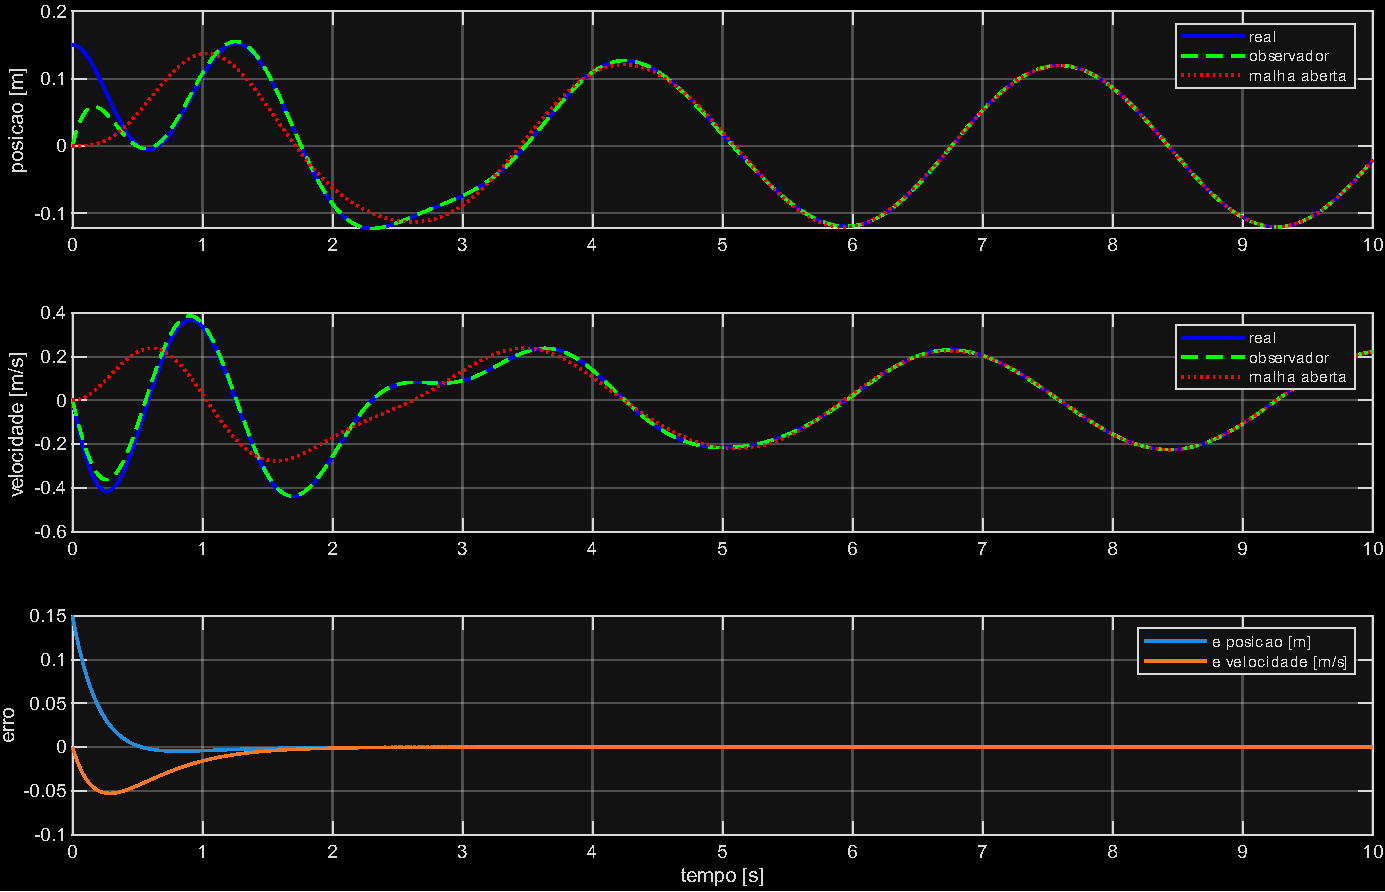
\includegraphics[width=\linewidth]{img/Estados e erro_3.pdf}
        \label{fig:estados3}
    \end{subfigure}
    \hfill
    \begin{subfigure}[b]{0.45\textwidth}
        \centering
        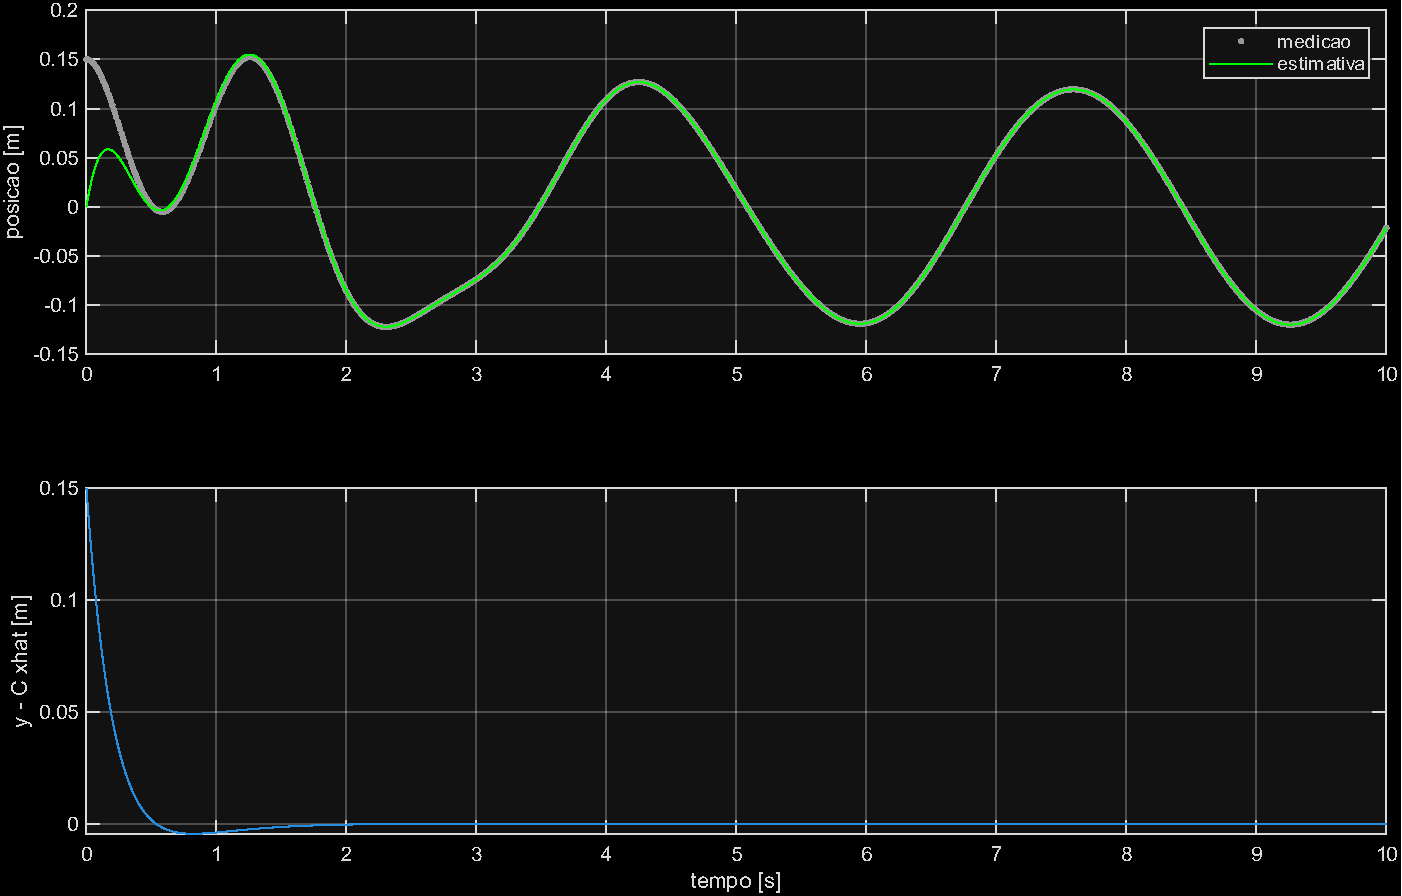
\includegraphics[width=\linewidth]{img/Medicao e inovacao_3.pdf}
        \label{fig:medicao3}
    \end{subfigure}
    \caption{Resultados da simulação com observador}
    \label{fig:ex3}
\end{figure}

\textbf{3.4)} $X(:,j)$ e $H(:,j)$ referem-se ao mesmo instante $t_j$.
        Comparar $X(:,j)$ com $H(:,j{+}1)$ introduziria um erro de
        desalinhamento $\approx T_s \dot{x}$, que não se anula (o sistema
        é sempre excitado por $u$), mesmo com um observador perfeito.

\noindent\textbf{4)}

\textbf{4.1)} Polos mais rápidos reduzem o transiente, mas exigem um ganho $L$ maior, amplificando o ruído, sobretudo na
velocidade.

\begin{table}[htbp]
    \centering
    \begin{minipage}[t]{0.35\textwidth}
        \hspace*{1em}\textbf{4.2)} O caso c converge mais depressa, mas tem pior RMSE em regime: é o compromisso rapidez--ruído.
    \end{minipage}
    \hfill
    \begin{minipage}[t]{0.60\textwidth}
        \vspace{0pt}
        \centering
        \caption{RMSE após 2 s.}
        \label{tab:polos}
        \begin{tabular}{lccc}\hline
        Caso & Polos & RMSE $p$ [m] & RMSE $v$ [m/s]\\\hline
        a ($\sigma=0$)    & $-3,-4$   & 6.181e-05 & 0.00016021\\
        b ($\sigma=0.03$) & $-3,-4$   & 0.0044406 & 0.023322\\
        c ($\sigma=0.03$) & $-12,-16$ & 0.011647  & 0.053313\\\hline
        \end{tabular}
    \end{minipage}
\end{table}

\begin{figure}[htbp]
    \centering
    \begin{minipage}[t]{0.45\textwidth}
        \vspace{0pt}
        \raggedright
        \hspace*{1em}\textbf{4.3)} \textbf{Azul:} massa real (só disponível em simulação); \textbf{verde:} estimativa
do observador; \textbf{vermelho:} réplica em malha aberta. Com ruído,
$y_j-C_d\hat x_j=C_de_j+n_j$: mesmo com $e=0$ a inovação fica igual ao ruído,
logo não tende para zero. 
    \end{minipage}
    \hfill
    \begin{minipage}[t]{0.45\textwidth}
        \vspace{0pt}
        \centering
        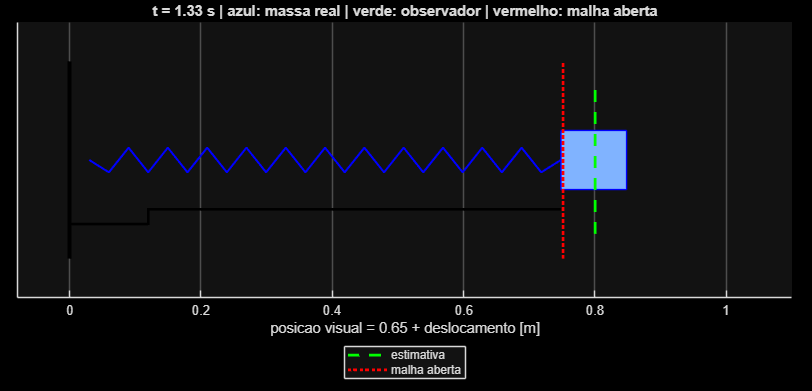
\includegraphics[width=\linewidth]{img/simul.png}
        \caption{Frame da animação.}
        \label{fig:estados}
    \end{minipage}
\end{figure}

\begin{figure}[htbp]
    \centering
    \begin{minipage}[t]{0.45\textwidth}
        \vspace{0pt}
        \raggedright
        \textbf{5)} Com $k_\text{real}=24$, subtraindo planta e observador: \[e_{j+1}=(A_d-LC_d)e_j+(A_r-A_d)x_j+(B_r-B_d)u_j\]
O termo forçado não se anula, porque $x$ e $u$ são sinusoidais, logo o erro
fica limitado mas não nulo (RMSE $\approx0.018$~m e $0.10$~m/s). Polos mais
rápidos reduzem-no, à custa de maior sensibilidade ao ruído.
    \end{minipage}
    \hfill
    \begin{minipage}[t]{0.45\textwidth}
        \vspace{0pt}
        \centering
        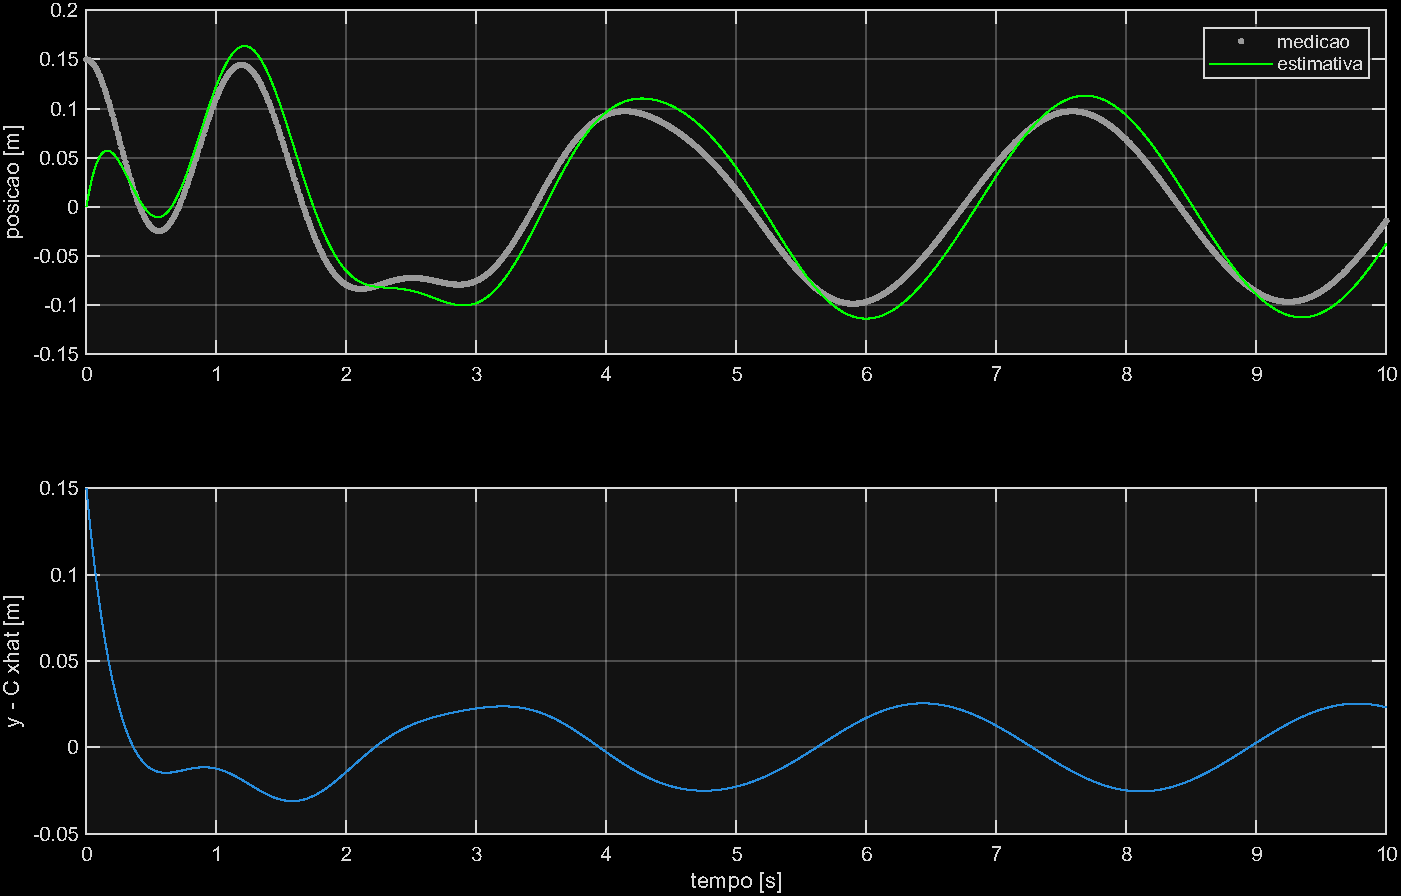
\includegraphics[width=\linewidth]{img/Medicao e inovacao_5.pdf}
        \caption{Medição e inovação com $k_\text{real}=24$}
        \label{fig:estados}
    \end{minipage}
\end{figure}













\printglossaries


\end{document}
